\section{HYPEBOL}
\subsection{KIẾN THỨC TRỌNG TÂM}
\subsubsection{Hình dạng của hypebol}
\begin{center}
    \begin{tikzpicture}[>=stealth,scale=.55, line join=round, line cap=round,font=\scriptsize]
        \draw[->] (-8,0)--(0.25,0)node[below left]{$ O $}--(8,0) node [below]{$x$};
        \draw[->] (0,-5.5)--(0,6) node [left]{$y$};
        %Hypebol
        \clip (-8,-5) rectangle (8,5);
        \draw[orange,thick,smooth,samples=100,domain=4:8] plot(\x,{3*sqrt(\x*\x/16-1)});
        \draw[orange,thick,smooth,samples=100,domain=-4:-8] plot(\x,{3*sqrt(\x*\x/16-1)});
        \draw[orange,thick,smooth,samples=100,domain=4:8] plot(\x,{-3*sqrt(\x*\x/16-1)});
        \draw[orange,thick,smooth,samples=100,domain=-4:-8] plot(\x,{-3*sqrt(\x*\x/16-1)});
        %Hình chữ nhật cơ sở
        \draw [dashed] (-4,-3)--(-4,3)--(4,3)--(4,-3)--(-4,-3);
        %Đường tiệm cận
        \draw[thin,smooth,blue,samples=100,domain=-8:8] plot(\x,{-(3/4)*\x});
        \draw (-5,3.5)node[above right]{$ y=-\dfrac{b}{a}x $};
        \draw[thin,smooth,blue,samples=100,domain=-8:8] plot(\x,{(3/4)*\x});
        \draw (5,3.5)node[above left]{$ y=\dfrac{b}{a}x $};
        %Đỉnh
        \draw [fill=black] (-4,0)node[above right]{$ A_1 $}circle(1.5pt) (4,0)node[above left]{$ A_2 $}circle(1.5pt) (-5,0)node[above]{$ F_1 $}circle(1.5pt) (5,0)node[above]{$ F_2 $}circle(1.5pt) (0,3)node[above left]{$ b $}circle(1.5pt) (0,-3)node[below left]{$ -b $}circle(1.5pt) (-4,0)node[below right]{$ -a $} (4,0)node[below left]{$ a $} (-5,0)node[below]{$ -c $} (5,0)node[below]{$ c $} (0,0)circle(1.5pt) (-4,-3)circle(1.5pt) (-4,3)circle(1.5pt) (4,-3)circle(1.5pt) (4,3)circle(1.5pt);
    \end{tikzpicture}
\end{center}
Cho hypebol có phương trình chính tắc $ \dfrac{x^2}{a^2}-\dfrac{y^2}{b^2}=1 $. Khi đó
\begin{itemize}
    \item Hypebol có hai \textbf{trục đối xứng} là $ Ox $ và $ Oy $, và có \textbf{tâm đối xứng} là gốc tọa độ $ O $.
    \item Trục $ Ox $ (chứa hai tiêu điểm) cắt hypebol tại hai điểm $ A_1(-a; 0) $, $ A_2(a; 0) $ và được gọi là \textbf{trục thực}.
    \item Hai điểm $ A_1(-a; 0) $, $ A_2(a; 0) $ được gọi là hai đỉnh.
    \item Trục đối xứng $ Oy $ không cắt hypebol và được gọi là \textbf{trục ảo}.
    \item $ 2a $, $ 2b $ tương ứng được gọi là \textbf{độ dài trục} thực,  trục ảo.
    \item Trong hai nhánh của hypebol, một nhánh chứa các điểm đều  có hoành độ $ x\ge a $ (nhánh chứa đỉnh $ A_2(a; 0) $), nhánh còn lại chứa các điểm đều có hoành độ $ x\le -a $ (nhánh chứa đỉnh $ A_1(-a; 0) $).
    \item Hình chữ nhật với bốn đỉnh có tọa độ là $ (-a; b) $, $ (-a; -b) $, $ (a; -b) $, $ (a; b) $ được gọi là \textbf{hình chữ nhật cơ sở}.
    \item Hai đường thẳng chứa hai đường chéo của hình chữ nhật cơ sở được gọi là hai \textbf{đường tiệm cận}, và có phương trình là $ y=-\dfrac{b}{a}x $ và $ y=\dfrac{b}{a}x $.
\end{itemize}
\begin{note}
    \textbf{Chú ý.}
    Trong hypebol nói trên, nhánh chứa đỉnh $ A_2(a; 0) $ là nhánh gồm các điểm $ M $ thỏa mãn $ MF_1-MF_2=2a $, nhánh chứa đỉnh $ A_1(-a; 0) $ là nhánh gồm các điểm $ M $ thỏa mãn $ MF_2-MF_1=2a $ (với $ F_1(-c; 0) $, $ F_2(c; 0) $ là các \textbf{tiêu điểm}, $ c=\sqrt{a^2+b^2} $).\\
    \textbf{Tiêu cự} $ 2c $ là khoảng cách giữa hai tiêu điểm.
\end{note} 
\subsubsection{Bán kính qua tiêu}
Cho hypebol có phương trình chính tắc $ \dfrac{x^2}{a^2}-\dfrac{y^2}{b^2}=1 $ với các tiêu điểm $ F_1(-c; 0) $, $ F_2(c; 0) $ (với $ c=\sqrt{a^2+b^2} $). Với điểm $ M(x; y) $ thuộc hypebol, ta có 
$$ MF_1=\left|a+\dfrac{c}{a}x\right|,\ MF_2=\left|a-\dfrac{c}{a}x\right|. $$
Các đoạn thẳng $ MF_1 $, $ MF_2 $ được gọi là \textbf{bán kính qua tiêu} của điểm $ M $.
\subsubsection{Tâm sai và đường chuẩn}
\immini{
    Cho hypebol có phương trình chính tắc $ \dfrac{x^2}{a^2}-\dfrac{y^2}{b^2}=1 $ với các tiêu điểm $ F_1(-c; 0) $, $ F_2(c; 0) $.\\
    Khi điểm $ M $ thay đổi trên hypebol, ta luôn có $ \dfrac{MF_1}{\mathrm{d}(M,\Delta_1)}=\dfrac{MF_2}{\mathrm{d}(M,\Delta_2)}=e $ không đổi, trong đó
    \begin{itemize}
        \item $ e=\dfrac{c}{a} $ được gọi là \textbf{tâm sai} của hypebol.
        \item $ \Delta_1\colon x=-\dfrac{a}{e} $ và $ \Delta_2\colon x=\dfrac{a}{e} $ được gọi là các \textbf{đường chuẩn} tương ứng với $ F_1(-c; 0) $ và $ F_2(c; 0) $ của hypebol.
    \end{itemize}
}{
    \begin{tikzpicture}[>=stealth,scale=.35, line join=round, line cap=round,font=\scriptsize]
        \draw[->] (-8,0)--(0.4,0)node[below left]{$ O $}--(8,0) node [below]{$x$};
        \draw[->] (0,-5.5)--(0,6) node [left]{$y$};
        %Hypebol
        \clip (-8,-5) rectangle (8,5);
        \draw[thick,smooth,samples=100,domain=4:8] plot(\x,{3*sqrt(\x*\x/16-1)});
        \draw[thick,smooth,samples=100,domain=-4:-8] plot(\x,{3*sqrt(\x*\x/16-1)});
        \draw[thick,smooth,samples=100,domain=4:8] plot(\x,{-3*sqrt(\x*\x/16-1)});
        \draw[thick,smooth,samples=100,domain=-4:-8] plot(\x,{-3*sqrt(\x*\x/16-1)});
        %Đường chuẩn
        \draw [ultra thick] (-3.2,-6)--(-3.2,6) (3.2,-5.5)--(3.2,6);
        \draw (-3.2,-4)node[right]{$ \Delta_1 $};
        \draw (3.2,-4)node[left]{$ \Delta_2 $};
        %Đường tiệm cận
        \draw[thin,smooth,samples=100,domain=-8:8] plot(\x,{-(3/4)*\x});
        \draw[thin,smooth,samples=100,domain=-8:8] plot(\x,{(3/4)*\x});
        %Khoảng cách
        \draw [orange,thick] (5,0)--(6,3.354)--(-5,0);
        \draw [blue,thick] (-3.2,3.354)--(6,3.354);
        %Đỉnh
        \draw [fill=black] (-4,0)circle(1.5pt)  (4,0)circle(1.5pt) (-5,0)node[below]{$ F_1 $}circle(1.5pt) (5,0)node[below]{$ F_2 $}circle(1.5pt) (-3.2,3.354)circle(2pt) (3.2,3.354)circle(2pt);
        %Điểm nằm trên hypebol
        \draw [fill=black] (6,3.354)node[below right]{$ M $}circle(2pt);
        %Đánh dấu góc vuông
        \newcommand{\gv}[4][black]{\draw[#1] ($ (#3)!8pt!(#2) $)--($ (#3)!2!($ ($ (#3)!8pt!(#2) $)!.5!($ (#3)!8pt!(#4) $) $) $)--($ (#3)!8pt!(#4) $);}
        \coordinate (A) at (-3.2,3.4);
        \coordinate (B) at (-3.2,3.354);
        \coordinate (C) at (3.2,3.4);
        \coordinate (D) at (3.2,3.354);
        \coordinate (M) at (6,3.354);
        \gv{A}{B}{M}
        \gv{C}{D}{M}
    \end{tikzpicture}
}
\subsection{CÁC DẠNG BÀI TẬP}
\begin{dang}{Xác định các yếu tố của Hypebol}
\end{dang}
\subsubsection{Các ví dụ}
\begin{vd}
    Cho hypebol $ \dfrac{x^2}{9}-\dfrac{y^2}{16}=1 $.
    \begin{enumerate}
        \item Tìm độ dài các trục và tọa độ các đỉnh.
        \item Tìm các đường tiệm cận.
    \end{enumerate}
    \loigiai{
        Từ phương trình của hypebol, ta có $ \heva{&a^2=9\\&b^2=16}\Rightarrow\heva{&a=3\\&b=4.} $
        \begin{enumerate}
            \item Hypebol có độ dài trục thực là $ 2a=6 $, độ dài trục ảo là $ 2a=8 $, và hai đỉnh là $ A_1(-3; 0) $, $ A_2(3; 0) $.
            \item Hypebol có hai đường tiệm cận là $ y=-\dfrac{4}{3}x $ và $ y=\dfrac{4}{3}x $.
        \end{enumerate}
    }
\end{vd}

\begin{vd}
    Cho hypebol $ \dfrac{x^2}{4}-\dfrac{y^2}{21}=1 $. Tính độ dài hai bán kính qua tiêu của một điểm $ M $ thuộc hypebol và có hoành độ bằng $ -10 $.
    \loigiai{
        Ta có $ \heva{&a^2=4\\&b^2=21}\Rightarrow\heva{&a=2\\&b=\sqrt{21}}\Rightarrow c=\sqrt{a^2+b^2}=5 $.\\ Do đó, hypebol có hai tiêu điểm là $ F_1(-5; 0) $, $ F_2(5; 0) $.\\
        Điểm $ M $ thuộc hypebol và có hoành độ $ x_0=-10 $ nên $$ MF_1=\left|a+\dfrac{c}{a}x_0\right|=\left|2+\dfrac{5}{2}\cdot(-10)\right|=23\text{ và } MF_2=\left|a-\dfrac{c}{a}x_0\right|=\left|2-\dfrac{5}{2}\cdot(-10)\right|=27. $$
    }
\end{vd}

\begin{vd}
    Cho hypebol có phương trình chính tắc $ \dfrac{x^2}{a^2}-\dfrac{y^2}{b^2}=1 $. Tìm điểm $ M $ trên hypebol để khoảng cách từ  $ M $ đến tiêu điểm $ F_2(c; 0) $ nhỏ nhất.
    \begin{center}
        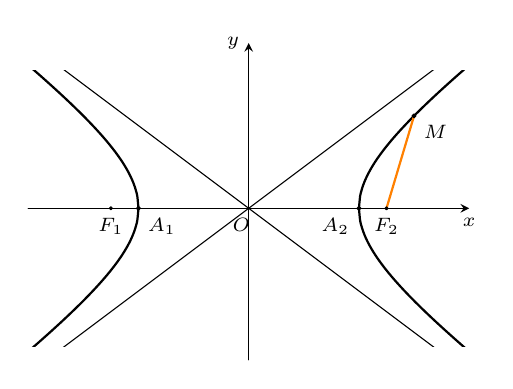
\begin{tikzpicture}[>=stealth,scale=.35, line join=round, line cap=round,font=\scriptsize]
            \draw[->] (-8,0)--(0.4,0)node[below left]{$ O $}--(8,0) node [below]{$x$};
            \draw[->] (0,-5.5)--(0,6) node [left]{$y$};
            %Hypebol
            \clip (-8,-5) rectangle (8,5);
            \draw[thick,smooth,samples=100,domain=4:8] plot(\x,{3*sqrt(\x*\x/16-1)});
            \draw[thick,smooth,samples=100,domain=-4:-8] plot(\x,{3*sqrt(\x*\x/16-1)});
            \draw[thick,smooth,samples=100,domain=4:8] plot(\x,{-3*sqrt(\x*\x/16-1)});
            \draw[thick,smooth,samples=100,domain=-4:-8] plot(\x,{-3*sqrt(\x*\x/16-1)});
            %Đường tiệm cận
            \draw[thin,smooth,samples=100,domain=-8:8] plot(\x,{-(3/4)*\x});
            \draw[thin,smooth,samples=100,domain=-8:8] plot(\x,{(3/4)*\x});
            %Khoảng cách
            \draw [orange,thick] (5,0)--(6,3.354);
            %Đỉnh
            \draw [fill=black] (-4,0)circle(1.5pt)  (4,0)circle(1.5pt) (-5,0)node[below]{$ F_1 $}circle(1.5pt) (5,0)node[below]{$ F_2 $}circle(1.5pt) (-4,0)node[below right]{$ A_1 $}circle(2pt) (4,0)node[below left]{$ A_2 $}circle(2pt);
            %Điểm nằm trên hypebol
            \draw [fill=black] (6,3.354)node[below right]{$ M $}circle(2pt);
        \end{tikzpicture}
    \end{center}
    \loigiai{
        Với mỗi điểm $ M(x_0; y_0) $ thuộc hypebol, ta có bán kính qua tiêu của $ M $ ứng với tiêu điểm $ F_2 $ là $ MF_2=\left|a-\dfrac{c}{a}x_0\right| $.
        \begin{itemize}
            \item Nếu $ M(x_0; y_0) $ thuộc nhánh chứa đỉnh $ A_2(a; 0) $ thì $ x_0\ge a $ nên $ a-\dfrac{c}{a}x_0<0 $ (để ý rằng $ c>a $). Do đó, $ MF_2=\left|a-\dfrac{c}{a}x_0\right|=\dfrac{c}{a}x_0-a\ge\dfrac{c}{a}a-a=c-a $.\\
            Dấu đẳng thức xảy ra khi $ x_0=a $, tức là, khi $ M(x_0; y_0) $ trùng đỉnh $ A_2(a;0) $.
            \item Nếu $ M(x_0; y_0) $ thuộc nhánh chứa đỉnh $ A_1(-a; 0) $ thì $ x_0\le -a $ nên $$  a-\dfrac{c}{a}x_0\ge a-\dfrac{c}{a}\cdot(-a)=a+c. $$ Do đó, $ MF_2=\left|a-\dfrac{c}{a}x_0\right|\ge a+c $.
        \end{itemize}
        Vậy điểm $ M(x_0; y_0) $ thuộc hypebol có khoảng cách tới tiêu điểm $ F_2(c; 0) $ nhỏ nhất khi $ M $ trùng đỉnh $ A_2(a; 0) $, và khi đó, khoảng cách bằng $ c-a $.
    }
\end{vd}
\begin{vd}
    Tìm tâm sai và các đường chuẩn của hypebol $ \dfrac{x^2}{64}-\dfrac{x^2}{17}=1 $.
    \loigiai{
        Ta có $ \heva{&a^2=64\\&b^2=17}\Rightarrow \heva{&a=8\\&b=\sqrt{17}} $ và $ c=\sqrt{a^2+b^2}=9 $.\\ Do đó, hypebol có tâm sai là $ e=\dfrac{c}{a}=\dfrac{9}{8} $ và các đường chuẩn là $ \Delta_1\colon x=-\dfrac{64}{9} $ (ứng với tiêu điểm $ F_1(-9; 0) $) và $ \Delta_2\colon x=\dfrac{64}{9} $ (ứng với tiêu điểm $ F_2(9; 0) $).
    }
\end{vd}

\subsubsection{Bài tập tương tự}
\begin{bt}
    Cho hypebol $ \dfrac{x^2}{64}-\dfrac{y^2}{36}=1 $
    \begin{enumerate}
        \item Tìm tiêu cự và độ dài các trục.
        \item Tìm các đỉnh và các đường tiệm cận.
    \end{enumerate}
    \loigiai{
        Ta có $ \heva{&a^2=64\\&b^2=36}\Rightarrow a=8, b=6, c=\sqrt{a^2+b^2}=10 $.\\
        \begin{enumerate}
            \item Hypebol có tiêu cự là $ 2c=20 $, độ dài trục thực là $ 2a=16 $, độ dài trục ảo là $ 2b=12 $.
            \item Các đỉnh của hypebol là $ A_1(-8,0) $, $ A_2(8,0) $.\\
            Các đường tiệm cận của hypebol là $ y=-\dfrac{3}{4}x $ và $ y=\dfrac{3}{4}x $.
        \end{enumerate}
    }
\end{bt}
\begin{bt}
    Cho hypebol có độ dài trục thực bằng $ 6 $, độ dài trục ảo bằng $ 6\sqrt3 $. Tính độ dài hai bán kính qua tiêu của một điểm $ M $ thuộc hypebol và có hoành độ bằng $ 9 $.
    \loigiai{
        Ta có $ \heva{&2a=6\\&2b=6\sqrt3}\Rightarrow\heva{&a=3\\&b=3\sqrt3\\&c=\sqrt{a^2+b^2}=6.} $\\
        Điểm $ M $ thuộc hypebol và có hoành độ $ x_0=9 $ nên $$ MF_1=\left|a+\dfrac{c}{a}x_0\right|=\left|3+\dfrac{6}{3}\cdot9\right|=21\text{ và } MF_2=\left|a-\dfrac{c}{a}x_0\right|=\left|3-\dfrac{6}{3}\cdot9\right|=15. $$
    }
\end{bt}
\begin{bt}
    Cho hypebol có phương trình chính tắc $ \dfrac{x^2}{a^2}-\dfrac{y^2}{b^2}=1 $. Tìm điểm $ M $ trên hypebol để khoảng cách từ  $ M $ đến tiêu điểm $ F_1(-c; 0) $ nhỏ nhất.
    \begin{center}
        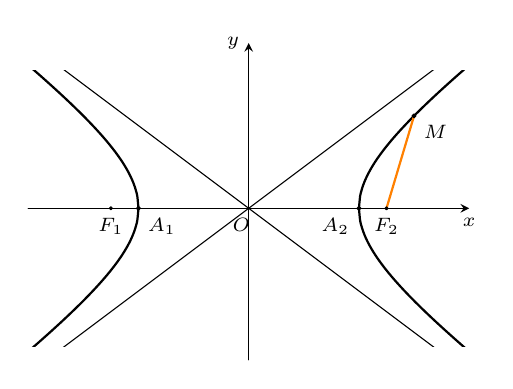
\begin{tikzpicture}[>=stealth,scale=.35, line join=round, line cap=round,font=\scriptsize]
            \draw[->] (-8,0)--(0.4,0)node[below left]{$ O $}--(8,0) node [below]{$x$};
            \draw[->] (0,-5.5)--(0,6) node [left]{$y$};
            %Hypebol
            \clip (-8,-5) rectangle (8,5);
            \draw[thick,smooth,samples=100,domain=4:8] plot(\x,{3*sqrt(\x*\x/16-1)});
            \draw[thick,smooth,samples=100,domain=-4:-8] plot(\x,{3*sqrt(\x*\x/16-1)});
            \draw[thick,smooth,samples=100,domain=4:8] plot(\x,{-3*sqrt(\x*\x/16-1)});
            \draw[thick,smooth,samples=100,domain=-4:-8] plot(\x,{-3*sqrt(\x*\x/16-1)});
            %Đường tiệm cận
            \draw[thin,smooth,samples=100,domain=-8:8] plot(\x,{-(3/4)*\x});
            \draw[thin,smooth,samples=100,domain=-8:8] plot(\x,{(3/4)*\x});
            %Khoảng cách
            \draw [orange,thick] (5,0)--(6,3.354);
            %Đỉnh
            \draw [fill=black] (-4,0)circle(1.5pt)  (4,0)circle(1.5pt) (-5,0)node[below]{$ F_1 $}circle(1.5pt) (5,0)node[below]{$ F_2 $}circle(1.5pt) (-4,0)node[below right]{$ A_1 $}circle(2pt) (4,0)node[below left]{$ A_2 $}circle(2pt);
            %Điểm nằm trên hypebol
            \draw [fill=black] (6,3.354)node[below right]{$ M $}circle(2pt);
        \end{tikzpicture}
    \end{center}
    \loigiai{
        Giải tương tự ví dụ 3, đáp án vẫn là $ c-a $.
    }
\end{bt}
\begin{bt}
    Cho hypebol $ \dfrac{x^2}{1}-\dfrac{y^2}{3}=1 $ với hai tiêu điểm $ F_1(-2; 0) $, $ F_2(2; 0) $. Điểm $ M $ nào thuộc hypebol mà có độ dài bán kính tiêu $ MF_2 $ nhỏ nhất? Tính khoảng cách từ điểm đó đến các tiêu điểm.
    \loigiai{
        Điểm $ M $ trùng với điểm $ A_2(1; 0) $. Khi đó, $ MF_1=1+(2)=3 $ và $ MF_2=2-1=1 $.
    }
\end{bt}

\begin{bt}
    Trong mặt phẳng tọa độ, cho hypebol có phương trình chính tắc $ \dfrac{x^2}{9}-\dfrac{y^2}{4}=1 $. Xác định tọa độ các đỉnh, độ dài các trục, tâm sai và phương trình các đường chuẩn của hypebol.
    \loigiai{
        Ta có $ \heva{&a^2=9\\&b^2=4}\Rightarrow a=3, b=2, c=\sqrt{a^2+b^2}=\sqrt{13} $.\\
        Tọa độ hai đỉnh của hypebol là $ A_1(-3; 0) $, $ A_2(3; 0) $.\\
        Độ dài trục thực $ 2a=6 $, độ dài trục ảo $ 2b=4 $.\\
        Tâm sai $ e=\dfrac{c}{a}=\dfrac{\sqrt{13}}{3} $.\\
        Phương trình các đường chuẩn $ \Delta_1\colon x=-\dfrac{9\sqrt{13}}{13} $ và $ \Delta_2\colon x=\dfrac{9\sqrt{13}}{13} $.
    }
\end{bt}
\begin{bt}
    Trong mặt phẳng tọa độ, cho hypebol có phương trình chính tắc $ \dfrac{x^2}{9}-\dfrac{y^2}{7}=1 $. Tính bán kính qua tiêu của một điểm $ M $ thuộc hypebol và có hoành độ bằng $ 12 $.
    \loigiai{
        Ta có $ \heva{&a^2=9\\&b^2=7}\Rightarrow a=3, b=\sqrt7, c=\sqrt{a^2+b^2}=4 $.\\
        Điểm $ M $ thuộc hypebol và có hoành độ $ x_0=12 $ nên $$ MF_1=\left|a+\dfrac{c}{a}x_0\right|=\left|3+\dfrac{4}{3}\cdot12\right|=19\text{ và } MF_2=\left|a-\dfrac{c}{a}x_0\right|=\left|3-\dfrac{4}{3}\cdot12\right|=13. $$
    }
\end{bt}
\begin{bt}
    Một hypebol mà độ dài trục thực bằng độ dài trục ảo được gọi là hypebol vuông. Tìm tâm sai và phương trình hai đường tiệm cân của hypebol vuông.
    \loigiai{
        Giả sử hypebol $ \dfrac{x^2}{a^2}-\dfrac{y^2}{b^2}=1 $ là hypebol vuông. Khi đó $ a=b $.\\
        Ta có $ c=\sqrt{a^2+b^2}=a\sqrt 2 $.\\
        Tâm sai của hypebol vuông là $ e=\dfrac{a\sqrt2}{a}=\sqrt2 $.\\
        Phương trình hai đường chuẩn $ \Delta_1\colon x=-\dfrac{a^2\sqrt2}{2} $, $ \Delta_2\colon x=\dfrac{a^2\sqrt2}{2} $.
    }
\end{bt}
\begin{dang}{Viết phương trình chính tắc của Hypebol}
\end{dang}
\subsubsection{Ví dụ minh họa}
\begin{vd}
    Trong mặt phẳng tọa độ $ Oxy $, hypebol $ (H) $ có phương trình chính tắc, đi qua điểm $ A(4; 0) $ và có tâm sai $ e=3 $. Tìm phương trình chính tắc của $ (H) $.
    \loigiai{
        Phương trình chính tắc của hypebol có dạng $$ \dfrac{x^2}{a^2}-\dfrac{y^2}{b^2}=1. $$
        Vì hypebol đi qua điểm $ A(4; 0) $ nên ta có $$ \dfrac{16}{a^2}-\dfrac{0^2}{b^2}=1\Rightarrow a^2=16\Rightarrow a=4. $$
        Theo công thức tính tâm sai ta có $$ e=\dfrac{c}{a}=3\Rightarrow c=3a=3\cdot 4=12. $$
        Do đó $ b^2=c^2-a^2=12^2-4^2=128 $.\\
        Vậy phương trình chính tắc của hypebol là $ \dfrac{x^2}{16}-\dfrac{y^2}{128}=1 $.
    }
\end{vd}
\begin{vd}
    Trong mặt phẳng tọa độ $ Oxy $, hypebol $ (H) $ có phương trình chính tắc, có một tiêu điểm là $ F_1(5; 0) $ và độ dài trục thực bằng $ 8 $.
    \loigiai{
        Vì $ (H) $ có một tiêu điểm $ F_1(5; 0) $ nên $ c=5 $.\\
        Độ dài trục thực của $ (H) $ bằng $ 8 $ nên $ 2a=8\Rightarrow a=4 $.\\
        Do đó $ b=\sqrt{c^2-a^2}=\sqrt{5^2-4^2}=3 $.\\
        Phương trình chính tắc của hypebol là $ \dfrac{x^2}{16}-\dfrac{y^2}{9}=1 $.
    }
\end{vd}

\begin{vd}
        Trong mặt phẳng tọa độ $ Oxy $, hypebol $ (H) $ có phương trình chính tắc, có tiêu điểm $ F_1(-\sqrt3; 0) $, một đường tiệm cận là $ y=\dfrac{2}{3}x $.
    \loigiai{
        Vì hypebol có tiêu điểm $ F_1(-\sqrt3; 0) $ nên $ c=\sqrt3 $.\\
        Hypebol có một đường tiệm cận là $ y=\dfrac{2}{3}x $ nên $ \dfrac{b}{a}=\dfrac{2}{3}\Rightarrow b=\dfrac{2a}{3} $.\\
        Ta có $ \begin{aligned}[t]
            c^2=a^2+b^2 &\Leftrightarrow 3=a^2+\dfrac{4a^2}{9}\\
                        &\Leftrightarrow a^2=\dfrac{27}{13}\Rightarrow b^2=3-\dfrac{27}{13}=\dfrac{12}{13}.
        \end{aligned} $\\
        Phương trình chính tắc của hypebol là $ \dfrac{x^2}{\frac{27}{13}}-\dfrac{y^2}{\frac{12}{13}}=1 $.
    }
\end{vd}

\subsubsection{Bài tập tương tự}
\begin{bt}
    Trong mặt phẳng tọa độ $ Oxy $, hypebol $ (H) $ có phương trình chính tắc, có tâm sai $ e=2 $ và một đường chuẩn là $ x=8 $. Lập phương trình chính tắc của $ (H) $.
    \loigiai{
        Hypebol có tâm sai $ e=2\Leftrightarrow \dfrac{c}{a}=2\Leftrightarrow c=2a. \ \ (1) $\\
        Hypebol có đường chuẩn là $ x=8\Rightarrow \dfrac{a^2}{c}=8\Leftrightarrow c=\dfrac{a^2}{8}.\ \ (2) $\\
        Từ $ (1) $ và $ (2) $, ta có hệ phương trình $ \heva{&c=2a\\&c=\dfrac{a^2}{8}}\Rightarrow\heva{&a=16\\&c=32}\Rightarrow b^2=c^2-a^2=768 $.\\
        Vậy phương trình chính tắc của $ (H) $ là $ \dfrac{x^2}{256}-\dfrac{y^2}{768}=1 $.
    }
\end{bt}
\begin{bt}
    Trong mặt phẳng tọa độ $ Oxy $, hypebol $ (H) $ có phương trình chính tắc. Lập phương trình chính tắc của $ (H) $ trong mỗi trường hợp sau:
    \begin{enumerate}
        \item $ (H) $ có nửa trục thực bằng $ 4 $, tiêu cự bằng $ 10 $.
        \item $ (H) $ có tiêu cự bằng $ 2\sqrt{13} $, một đường tiệm cận là $ y=\dfrac{2}{3}x $.
        \item $ (H) $ có tâm sai $ e=\sqrt5 $, và đi qua điểm $ (\sqrt{10}; 6) $.
    \end{enumerate}
    \loigiai{
        \begin{enumerate}
            \item Ta có $ \heva{&a=4\\&2c=10}\Leftrightarrow\heva{&a=4\\&c=5}\Rightarrow b=\sqrt{c^2-a^2}=3 $.\\
            Vậy phương trình chính tắc của $ (H) $ là $ \dfrac{x^2}{16}-\dfrac{y^2}{9}=1 $.
            \item Ta có $ \heva{&2c=2\sqrt{13}\\&\dfrac{b}{a}=\dfrac{2}{3}}\Leftrightarrow\heva{&c=\sqrt{13}\\&a=\dfrac{3b}{2}.} $\\
            Mà $ c^2=a^2+b^2\Leftrightarrow 13=\dfrac{9b^2}{4}+b^2\Leftrightarrow b^2=4, a^2=9 $.\\
            Vậy phương trình chính tắc của $ (H) $ là $ \dfrac{x^2}{9}-\dfrac{y^2}{4}=1 $.
            \item Giả $ (H) $ có phương trình chính tắc là $ \dfrac{x^2}{a^2}-\dfrac{y^2}{b^2}=1 $.\\
            $ (H) $ có tâm sai $ e=\sqrt5\Leftrightarrow\dfrac{c}{a}=\sqrt5\Leftrightarrow c=a\sqrt5 $.\\
            Mà $ c^2=a^2+b^2\Leftrightarrow 5a^2=a^2+b^2\Leftrightarrow b^2=4a^2 $.\\
            $ (H) $ đi qua $ (\sqrt{10};6) $ nên $ \dfrac{10}{a^2}-\dfrac{36}{b^2}=1\Leftrightarrow \dfrac{10}{a^2}-\dfrac{36}{4a^2}=1\Leftrightarrow a^2=1\Rightarrow b^2=4 $.\\
            Vậy phương trình chính tắc của $ (H) $ là $ \dfrac{x^2}{1}-\dfrac{y^2}{4}=1 $.
        \end{enumerate}
    }
\end{bt}
\Closesolutionfile{ans}
